\documentclass{standalone}
\usepackage{tikz}
\usetikzlibrary{patterns, positioning}
\usetikzlibrary{shapes.misc}
\usepackage[outline]{contour}
\contourlength{1.5pt} 


\begin{document}
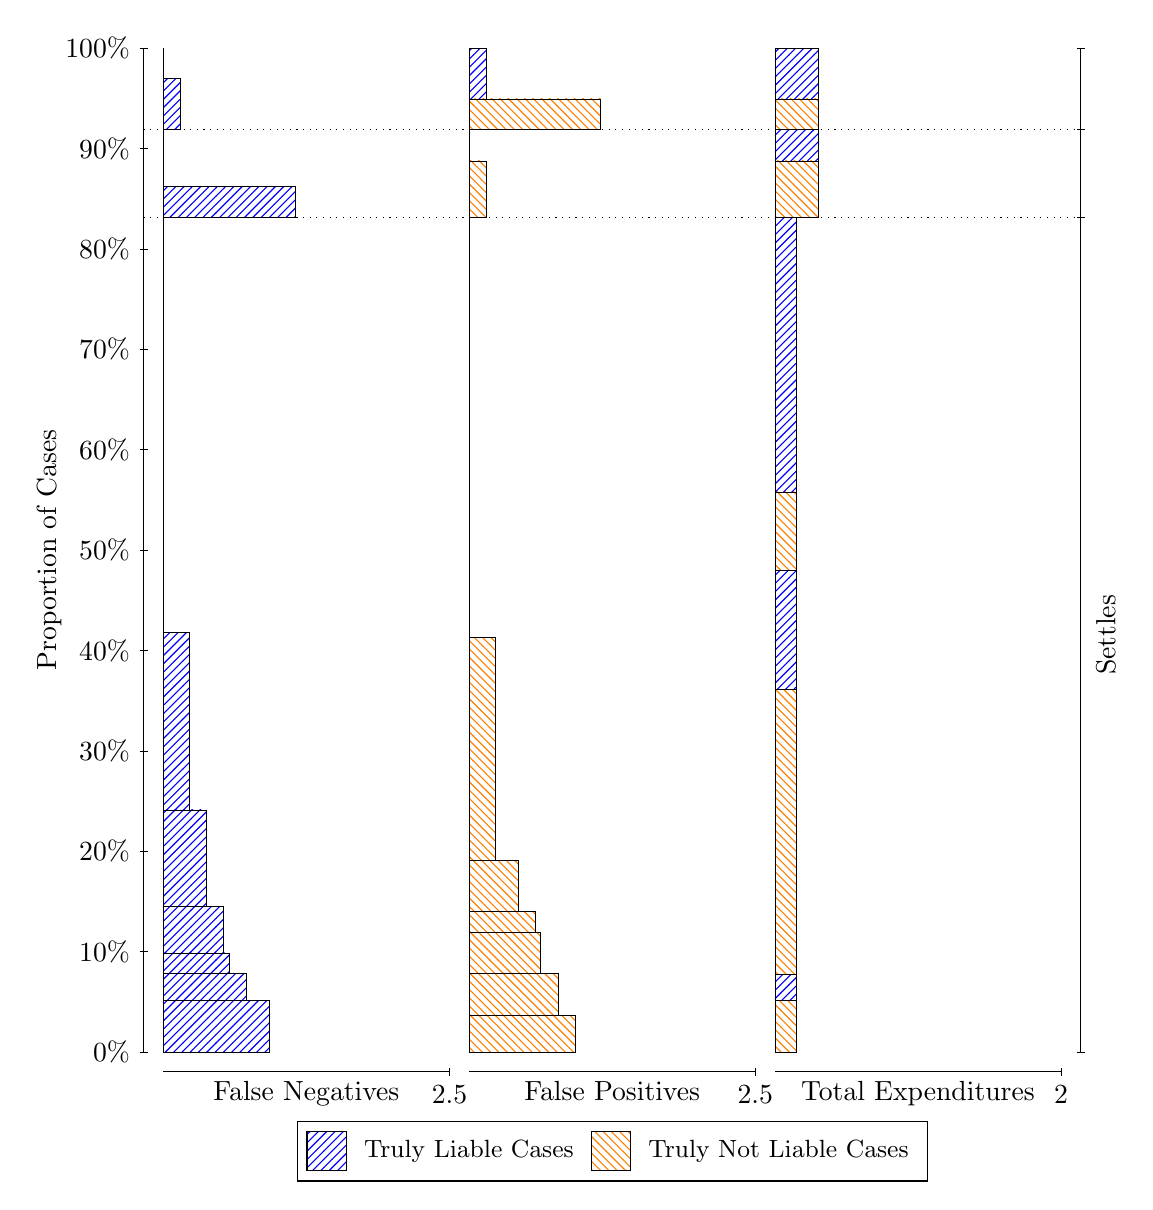
\begin{tikzpicture}
\draw[black, very thin] (1.5,1.75) -- (1.5,14.5);
\node[rotate=90, text=black, anchor=center] at (0.3, 8.125) {Proportion of Cases};
\draw[black, very thin] (1.45,1.75) -- (1.55,1.75);
\node[text=black, anchor=east] at (1.45, 1.75) {0\%};
\draw[black, very thin] (1.45,3.025) -- (1.55,3.025);
\node[text=black, anchor=east] at (1.45, 3.025) {10\%};
\draw[black, very thin] (1.45,4.3) -- (1.55,4.3);
\node[text=black, anchor=east] at (1.45, 4.3) {20\%};
\draw[black, very thin] (1.45,5.575) -- (1.55,5.575);
\node[text=black, anchor=east] at (1.45, 5.575) {30\%};
\draw[black, very thin] (1.45,6.85) -- (1.55,6.85);
\node[text=black, anchor=east] at (1.45, 6.85) {40\%};
\draw[black, very thin] (1.45,8.125) -- (1.55,8.125);
\node[text=black, anchor=east] at (1.45, 8.125) {50\%};
\draw[black, very thin] (1.45,9.4) -- (1.55,9.4);
\node[text=black, anchor=east] at (1.45, 9.4) {60\%};
\draw[black, very thin] (1.45,10.675) -- (1.55,10.675);
\node[text=black, anchor=east] at (1.45, 10.675) {70\%};
\draw[black, very thin] (1.45,11.95) -- (1.55,11.95);
\node[text=black, anchor=east] at (1.45, 11.95) {80\%};
\draw[black, very thin] (1.45,13.225) -- (1.55,13.225);
\node[text=black, anchor=east] at (1.45, 13.225) {90\%};
\draw[black, very thin] (1.45,14.5) -- (1.55,14.5);
\node[text=black, anchor=east] at (1.45, 14.5) {100\%};

\draw[black, very thin] (13.4,1.75) -- (13.4,14.5);
\draw[black, very thin] (13.35,1.75) -- (13.45,1.75);
\node[anchor=west] at (13.35, 1.75) {};
\draw[black, very thin] (13.35,12.345) -- (13.45,12.345);
\node[anchor=west] at (13.35, 12.345) {};
\draw[black, very thin] (13.35,13.47) -- (13.45,13.47);
\node[anchor=west] at (13.35, 13.47) {};
\draw[black, very thin] (13.35,14.5) -- (13.45,14.5);
\node[anchor=west] at (13.35, 14.5) {};

\draw[black, very thin, pattern color=blue, pattern=north east lines] (1.75,1.75) rectangle (3.0943,2.4101);
\draw[black, very thin, pattern color=blue, pattern=north east lines] (1.75,2.4101) rectangle (2.8037,2.7484);
\draw[black, very thin, pattern color=blue, pattern=north east lines] (1.75,2.7484) rectangle (2.5857,3.0098);
\draw[black, very thin, pattern color=blue, pattern=north east lines] (1.75,3.0098) rectangle (2.513,3.5972);
\draw[black, very thin, pattern color=blue, pattern=north east lines] (1.75,3.5972) rectangle (2.295,4.8254);
\draw[black, very thin, pattern color=blue, pattern=north east lines] (1.75,4.8254) rectangle (2.077,7.079);
\draw[black, very thin, pattern color=orange, pattern=north west lines] (1.75,7.079) rectangle (1.75,12.345);
\draw[black, very thin, pattern color=blue, pattern=north east lines] (1.75,12.345) rectangle (3.4213,12.746);
\draw[black, very thin, pattern color=orange, pattern=north west lines] (1.75,12.746) rectangle (1.75,13.47);
\draw[black, very thin, pattern color=blue, pattern=north east lines] (1.75,13.47) rectangle (1.968,14.114);
\draw[black, very thin, pattern color=orange, pattern=north west lines] (1.75,14.114) rectangle (1.75,14.5);
\draw[black, very thin, pattern color=orange, pattern=north west lines] (5.6333,1.75) rectangle (6.9777,2.2107);
\draw[black, very thin, pattern color=orange, pattern=north west lines] (5.6333,2.2107) rectangle (6.7597,2.7484);
\draw[black, very thin, pattern color=orange, pattern=north west lines] (5.6333,2.7484) rectangle (6.5417,3.2722);
\draw[black, very thin, pattern color=orange, pattern=north west lines] (5.6333,3.2722) rectangle (6.469,3.5336);
\draw[black, very thin, pattern color=orange, pattern=north west lines] (5.6333,3.5336) rectangle (6.251,4.1853);
\draw[black, very thin, pattern color=orange, pattern=north west lines] (5.6333,4.1853) rectangle (5.9603,7.0156);
\draw[black, very thin, pattern color=blue, pattern=north east lines] (5.6333,7.0156) rectangle (5.6333,12.345);
\draw[black, very thin, pattern color=orange, pattern=north west lines] (5.6333,12.345) rectangle (5.8513,13.068);
\draw[black, very thin, pattern color=blue, pattern=north east lines] (5.6333,13.068) rectangle (5.6333,13.47);
\draw[black, very thin, pattern color=orange, pattern=north west lines] (5.6333,13.47) rectangle (7.3047,13.855);
\draw[black, very thin, pattern color=blue, pattern=north east lines] (5.6333,13.855) rectangle (5.8513,14.5);
\draw[black, very thin, pattern color=orange, pattern=north west lines] (9.5167,1.75) rectangle (9.7892,2.4017);
\draw[black, very thin, pattern color=blue, pattern=north east lines] (9.5167,2.4017) rectangle (9.7892,2.74);
\draw[black, very thin, pattern color=orange, pattern=north west lines] (9.5167,2.74) rectangle (9.7892,6.3555);
\draw[black, very thin, pattern color=blue, pattern=north east lines] (9.5167,6.3555) rectangle (9.7892,7.8643);
\draw[black, very thin, pattern color=orange, pattern=north west lines] (9.5167,7.8643) rectangle (9.7892,8.8627);
\draw[black, very thin, pattern color=blue, pattern=north east lines] (9.5167,8.8627) rectangle (9.7892,12.345);
\draw[black, very thin, pattern color=orange, pattern=north west lines] (9.5167,12.345) rectangle (10.062,13.068);
\draw[black, very thin, pattern color=blue, pattern=north east lines] (9.5167,13.068) rectangle (10.062,13.47);
\draw[black, very thin, pattern color=orange, pattern=north west lines] (9.5167,13.47) rectangle (10.062,13.855);
\draw[black, very thin, pattern color=blue, pattern=north east lines] (9.5167,13.855) rectangle (10.062,14.5);
\draw[black, dotted] (1.5,12.345) -- (13.4,12.345);
\draw[black, dotted] (1.5,13.47) -- (13.4,13.47);
\draw[black, very thin] (1.75,1.5) -- (5.3833,1.5);
\node[text=black, anchor=north] at (3.5667, 1.5) {False Negatives};
\draw[black, very thin] (5.3833,1.45) -- (5.3833,1.55);
\node[text=black, anchor=north] at (5.3833, 1.45) {2.5};

\draw[black, very thin] (5.6333,1.5) -- (9.2667,1.5);
\node[text=black, anchor=north] at (7.45, 1.5) {False Positives};
\draw[black, very thin] (9.2667,1.45) -- (9.2667,1.55);
\node[text=black, anchor=north] at (9.2667, 1.45) {2.5};

\draw[black, very thin] (9.5167,1.5) -- (13.15,1.5);
\node[text=black, anchor=north] at (11.333, 1.5) {Total Expenditures};
\draw[black, very thin] (13.15,1.45) -- (13.15,1.55);
\node[text=black, anchor=north] at (13.15, 1.45) {2};

\node[text=black, centered, rotate=90] at (13.72, 7.0473) {\contour{white}{Settles}};



\draw (7.449999999999999,1.5) node[draw=none] (baseCoordinate) {};
\begin{scope}[align=center]
        \matrix[scale=0.5, draw=black, below=0.5cm of baseCoordinate, nodes={draw}, column sep=0.1cm]{
            \node[rectangle, draw, minimum width=0.5cm, minimum height=0.5cm, pattern color=blue, pattern=north east lines] {}; &
            \node[draw=none, font=\small, text=black] (B) {Truly Liable Cases}; &
            \node[rectangle, draw, minimum width=0.5cm, minimum height=0.5cm, pattern color=orange, pattern=north west lines] {}; &
            \node[draw=none, font=\small, text=black] (B) {Truly Not Liable Cases}; \\
            };
\end{scope}

\end{tikzpicture}
\end{document}